% This is a LaTeX file. It is a text file that is compiled
% by a program called LaTeX into a pretty PDF file.
% If you're viewing this file in Overleaf, you'll see that PDF
% in the window to the right.
%
% This file is for typesetting YOUR ANSWERS to this homework assignment.
% The LaTeX macro language is complicated, so we have inserted lots of
% documenting comments into the file. Comments start with '%'
% and continue to the end of the line. In Overleaf's edit window, they
% are colored green.
%
% Comments prefixed with 'Student:' are relevant to students. Skip any-
% thing else you don't understand, or ask me.

\documentclass{article}
%% This is some font management depending on the TeX “engine” being used.
%% Nothing to worry about.
\usepackage{ifxetex}
\ifxetex
  \usepackage{fontspec}
\else
  \usepackage[T1]{fontenc}
  \usepackage[utf8]{inputenc}
  \usepackage{lmodern}
\fi

%% Student: These lines describe some document metadata.
\title{Problem Set 2}
\usepackage{etoolbox}
\makeatletter\preto{\@title}{Answers to }\makeatother
\author{%
%% Student: change the next line to your name!
    Hongyi Zheng
\\  CSCI-UA 310 Basic Algorithms
}

%% These lines set up the question, answer, and solution environments.
\usepackage{amsthm}
\usepackage{amssymb}
\theoremstyle{plain}
\newtheorem{question}{Question}

\newenvironment{answer}[1][Answer]
    {\begin{proof}[#1]{$ $}\renewcommand\qedsymbol{$\vartriangle$}}
    {\end{proof}}
\newenvironment{solution}[1][Solution]
    {\begin{proof}[#1]{$ $}\renewcommand\qedsymbol{$\blacktriangleup$}}
    {\end{proof}}
\makeatletter
    \newcommand{\stepenumdepth}{\advance\@enumdepth\@ne}
\makeatother
\AtBeginEnvironment{question}{\stepenumdepth}
\AtBeginEnvironment{answer}{\stepenumdepth}
\AtBeginEnvironment{solution}{\stepenumdepth}

\usepackage{amsmath}
\usepackage{siunitx}
\DeclareSIUnit{\pound}{lb}
\usepackage{bm}

\usepackage{tikz}
\usetikzlibrary{calc}
\usepackage{caption,subcaption}

\usepackage{hyperref}
\usepackage{graphicx}
\usepackage{enumerate}
%% This is the beginning of the part of the file that describes
%% the actual text of the document.
%% That's why it says `\begin{document}' below. :-)
\begin{document}
\maketitle


\begin{question}
\end{question}
%% Student: put your answer between the next two lines.
\begin{answer}
    \begin{enumerate}
        Following these steps to find $k$ in $O(\log n)$:
        \begin{enumerate}
            \item  we compare $a_{\frac{n}{4}}$ and $a_{\frac{3n}{4}}$. If $a_{\frac{n}{4}} < a_{\frac{3}{4}n}$, then the shift point is not between $a_{\frac{n}{4}}$ and $a_{\frac{3}{4}n}$. If $a_{\frac{n}{4}} > a_{\frac{3}{4}n}$
            then the shift point is between $a_{\frac{n}{4}}$ and $a_{\frac{3}{4}n}$.
            \item We could rule out half of the array, and compare the number on the first quartile and that on the third quartile of the remaining array to further narrow the range.
            \item Repeating that process and we could find the index of $a_n$. If $a_n$ is the $i$th number in the array, then $k=n-i$
        \end{enumerate}
    \end{enumerate}
\end{answer}

\begin{question}
\end{question}
\begin{answer}
    \begin{enumerate}
        \item
        \begin{enumerate}
            \item
            Convert $[a_1 \cdots a_n]$ into $[b_0 \cdots b_n]$, where $\displaystyle b_0 = 0, b_1 = a_1, b_2 = a_1 + a_2, \cdots ,b_n = \sum_{i=1}^{n} a_i$.
            \item
            Since this the new array is sorted, except for $b_0$, for each $b_j$, we could use binary search to find a $b_i$ such that $b_j - b_{i-1} = s_{ij} < s$, but $b_j - b_{i-2} = s_{i-1j} > s$, and we could add $j-i+1$ to the total number of subarrays. If we found that even $b_j - b_0 < s$, then we simply add $j$ to the total number of subarrays.
            \item
            Add up the number of subarrays ending at different term in $[a_1 \cdots a_n]$, we get the total number of subarrays.
        \end{enumerate}
        \item
        \begin{enumerate}
            \item
            Adding up $a_1$, $a_2 \cdots a_{k_1}$ until $s_{1k_1} < s$, but $s_{1k_1+1} >= s$. We know that there are $k_1$ subarrays, $A_{11}, A_{12} \cdots A_{1k_1}$, starting from $a_1$ and satisfies $s_{ij} < s$.
            \item
            Next, remove $a_1$ from the sum and add terms after $a_{k_1}$ until $a_{k_2}$, such that $s_{2k_2} < s$, but $s_{2k_2+1} >= s$. We know that there are $k_2 - 1$ subarrays, $A_{22}, A_{23} \cdots A_{2k_2}$, starting from $a_2$ and satisfies $s_{ij} < s$.
            \item
            Keep repeating that process until we find the all numbers of subarrays starting from every term in the array. If we reach the end of the array when finding $a_{k_i}$, then just use the last term in the array as $a_{k_i}, a_{k_{i+1}} \cdots a_{k_n}$.
            \item
            During the process we add up the number of subarrays that starting from every single term in the array and satisfy $s_{ij} < s$. That sum is the total number of subarray that satisfies the requirement.
        \end{enumerate}
    \end{enumerate}
\end{answer}

\begin{question}
\end{question}
%% Student: put your answer between the next two lines.
\begin{answer}
    \begin{enumerate}
        We could treat vectors as points.\\

        Given a set of $n$ vectors, we could convert them into a set of $4n$ points after reflection. Then use the closets pair of point algorithm to find the closest pair of points among those $4n$ points. They are really just a pair of vectors $(v_1, v_2)$, and the pair of vectors that minimize the sum is in fact $(v_1, -v_2)$. That is because $v_1 - v_2 = v_1 + (-v_2)$. \\

        Finally, we check which reflection of $v_1$ and $v_2$ are in the original set of vectors (takes linear time) to determine the reflection.
    \end{enumerate}
\end{answer}

\begin{question}
\end{question}
%% Student: put your answer between the next two lines.
\begin{answer}
    \begin{enumerate}
        \item
        Convert $[a_1 \cdots a_n]$ into an array of points $\displaystyle [(1, a_1), (2, a_1 + a_2), (3, a_1 + a_2 + a-3) \cdots (n, \sum_{i=1}^{n} a_i)]$. The utility of the subarray $[a_l \cdots a_r]$ is just the square of the distance between $\displaystyle(l, \sum_{i=1}^{l} a_i)$ and $\displaystyle(r, \sum_{i=1}^{r} a_i)$.
        Use the closest pair of points algorithm to find the closest pair of points in that array of points, the subarray with minimum utility is just $[a_{x_1} \cdots a_{x_2}]$, where $x_1$, $x_2$ are the $x$-axis of two points in the closest pair.
        \item
        First, we convert the array in the same way as the previous question. Then, we use the convex hull algorithm to figure out the set of points that form the hull. The points that result in the maximum utility are apparently on the hull. (Could be proofed geometrically)\\

        Then, use rotating calipers technique to figure out the longest diagonal of the convex hull, which connects the pair of points with the largest distance, and the subarray with maximum utility is just $[a_{x_1} \cdots a_{x_2}]$, where $x_1$, $x_2$ are the $x$-axis of two points connected by the longest diagonal.
    \end{enumerate}
\end{answer}

\begin{question}
\end{question}
%% Student: put your answer between the next two lines.
\begin{answer}
    \begin{enumerate}
        Following these steps to draw the binary tree in $O(n\log^2 n)$.
        \begin{enumerate}
            \item
            We sort the points according to the $x$-axis and choose the point in the middle as the root to divide the remaining points into two clusters.
            \item
            Next, we sort those two clusters according to the angle between the line connecting the point to the root and the horizontal line. We choose two points, which are in the middle of that two sorted clusters. They are the roots of the subtrees under the root of the binary tree.
            \item
            By connecting the root of the binary tree and those two points, we split those two clusters into four smaller clusters of equal size. Repeat step $(ii)$ for each subtree root until the clusters only contain a single point. Then we get the binary tree we want without any intersecting edges.
        \end{enumerate}

    \end{enumerate}
\end{answer}

\begin{question}
\end{question}
%% Student: put your answer between the next two lines.
\begin{answer}
    \begin{enumerate}
        \item
        On the levels where array size are equal to or greater than $2^l$, this has no effect on the number of cross sorted pairs. \\
        On the levels where array sizes are less than $2^l$, suppose the array size is $2^k$, then the number of the cross sorted pairs in each node on that level would be $n^\prime = 2^{2k} - n$, where $n$ is the number of the cross sorted pairs before flip.
        \item
        Flip operation swap those two numbers on the level where the array sizes are less than $2^l$ \\

        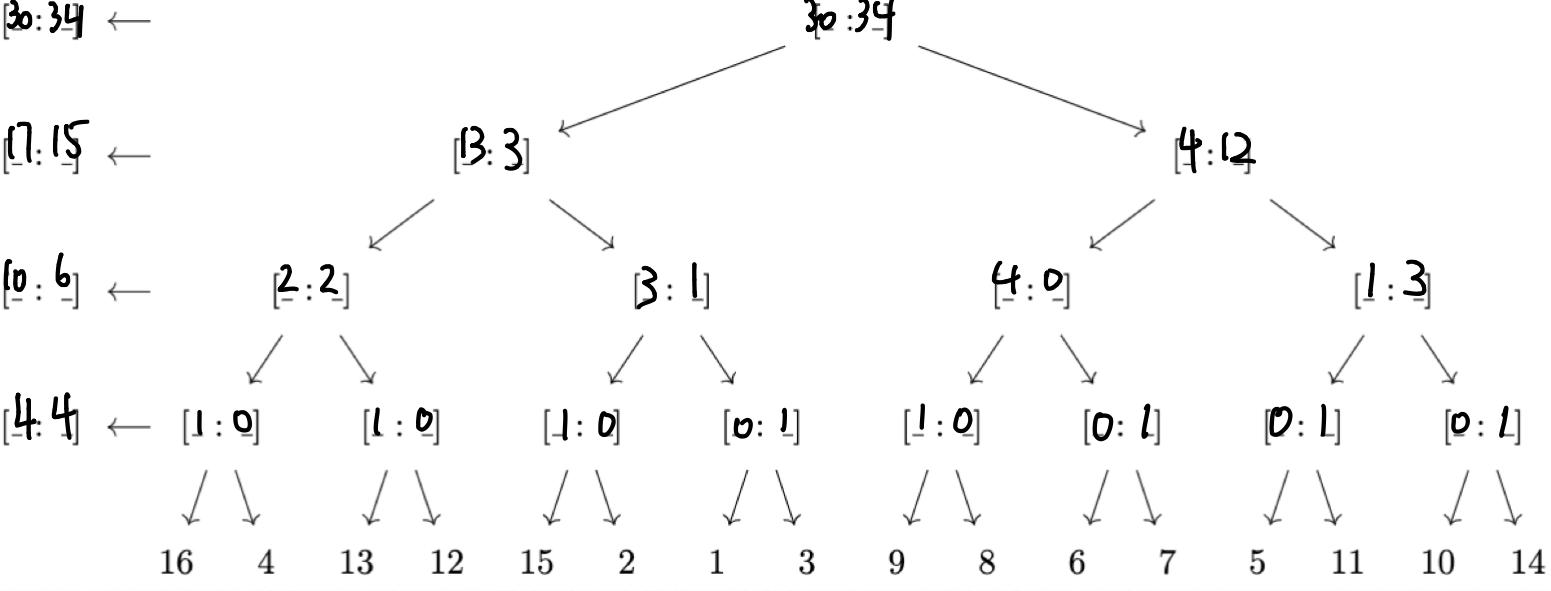
\includegraphics[width=0.9\columnwidth]{Q6_2.jpeg}
        \item
        \begin{enumerate}
            \item
            We first use the merge sort algorithm to figure out the number of cross inversion and the number of cross sorted pair at each node. We could sum up the those numbers if they belong to node in the same level. We use a tuple array of length $k + 1$ to store the number of cross inversion and the cross sorted pairs at each level. The first tuple saves the number of cross inversion and the cross sorted pairs at the base level, where the array length is $2^0 = 1$, and the last tuple saves those at the top level, where the array length is $2^k$.
            \item
            Swap the number of cross inversion and cross sorted pair in the first $l_1$ tuples. On these levels, the array size ranges from $2^0$ to $2^{l_1 - 1}$. Then sum up the number of cross inversions in each term of the array. Add that total number of inversions to the result array.
            \item
            Repeat that process, Swap the number of cross inversion and cross sorted pair in the first $l_i$ tuples, and after each operation calculate the total number of cross inversion and add the sum to the result array.
        \end{enumerate}
    \end{enumerate}
\end{answer}

\begin{question}
\end{question}
%% Student: put your answer between the next two lines.
\begin{answer}
    \begin{enumerate}
        \item
        If a number appears $n$ times in $[a_l \cdots a_r]$, then after sorting, the index of that number must also appear $n$ times. In contrast, if two terms are different, then their index will also be different after sorting. Thus, $u(1, i, a_i) = u(1, i, b_i)$, and $u(j, n, a_j) = u(j, n, b_j)$ where $b_i, b_j$ is the index of $a_i, a_j$. \\

        To convert them in $O(n\log n)$, we first copy the original array and sort the copy, which takes $O(n\log n)$. Then, iterating through sorted array to give every number an index and convert the unsorted original array into an index array, which both takes $O(n)$, and the total complexity is $O(n\log n)$
        \item
        \begin{enumerate}
            \item
            To create those arrays in $O(n)$, those two arrays will be filled separately.
            \item
            We begin from the \textbf{lreg} array. When filling the \textbf{lreg} array, we create another counter array with length equal to the max index, and every term of the array is $0$.
            \item
            Iterate through the \textbf{lreg} array, when we are processing a term, we check the corresponding counter in the counter array, increase that counter by one and fill that number in the \textbf{lreg}. For example, if the $i$th item is $2$, and the second item in the counter array is $3$, we increase $3$ by $1$ to $4$, and $u(1, i, a_i) = 4$.
            \item
            Similarly, iterate through the \textbf{rreg} array, but in the reverse order to fill it.
        \end{enumerate}
        \item
        \begin{enumerate}
            \item
            Follow the steps in previous questions to create \textbf{lreg} and \textbf{rreg} array, which takes $O(n\log n)$
            \item
            We could count the total number of cross inversions from \textbf{lreg} to \textbf{rreg} when mergesorting them, and that is the number of dominant pairs.
            \item
            Suppose we have the left halves and right halves of both arrays sorted, then before merging the left part of \textbf{lreg} and \textbf{rreg} with their right parts respectively, we need to count number of cross inversions from the left part of \textbf{lreg} to the right part of \textbf{rreg}, which is related to the number of dominant pairs. \\

            For example, we have
            \begin{equation*}
                \begin{aligned}
                    lreg &= 1\,2\,1\,1\quad1\,2\,1\,2 \\
                    rreg &= 2\,1\,2\,2\quad1\,1\,1\,1
                \end{aligned}
            \end{equation*}
            Then, after their left and right halves are sorted, they will become
            \begin{equation*}
                \begin{aligned}
                    lreg &= 1\,1\,1\,2\quad1\,1\,2\,2 \\
                    rreg &= 1\,2\,2\,2\quad1\,1\,1\,1
                \end{aligned}
            \end{equation*}
            We need to add the cross inversions between the left part of \textbf{lreg}, which is $[1, 1, 1, 2]$ and right part of the \textbf{rreg}, which is $[1, 1, 1, 1]$ to the total number of cross inversions. This process is similar to merging to sorted lists during a single list merge sort. When the current candidates in the two lists are equal, we will add the candidate from the left part of the \textbf{lreg}. In this case, we will put first three $1$s in the $[1, 1, 1, 2]$ to the merged list, and put all four $1$s in the $[1, 1, 1, 1]$ to the merged list, and finally put the $2$ into the merged list. During this process, we counted the number of cross inversions between left part of \textbf{lreg} and right part of the \textbf{rreg}, and add that count to the total number of the total number of cross inversion from \textbf{lreg} to \textbf{rreg}. In this case, we add 4 to the total count.
            \item
            We then mergesort \textbf{lreg} and \textbf{rreg} respectively, return two sorted arrays. By recursively mergesorting those two arrays and count cross inversion between left part of the subarray from \textbf{lreg} and right part of the subarray from \textbf{rreg} before merging \textbf{lreg} and \textbf{rreg} respectively, we could get the total number of cross inversion from \textbf{lreg} to \textbf{rreg}, which is the number of dominant pairs. 
        \end{enumerate}
    \end{enumerate}
\end{answer}

\end{document}
\endinput
%%
%% End of file `ps2.ans.tex'.
